 %%%%%%%%%%%%%%%%%%%%%%%%%%%%%%%%%%%%%%%%%%%%%%%%%%%%%%%%%%%%
%%
%% LaTeX Thesis Template defined by Torsten Schön, May 2013
%%
%%%%%%%%%%%%%%%%%%%%%%%%%%%%%%%%%%%%%%%%%%%%%%%%%%%%%%%%%%%%
\documentclass[letterpaper,11pt,twoside,openright]{report}

% define marging document
\usepackage[letterpaper,left=3cm,right=2cm,top=2cm,bottom=2cm]{geometry}

% define font arial
\usepackage{helvet}

\renewcommand{\familydefault}{\sfdefault}

% define spanish language and table name
\usepackage[spanish,es-tabla]{babel}

\usepackage[utf8]{inputenc}

\usepackage[T1]{fontenc}

% import graphics
\usepackage{graphicx}

\graphicspath{{fig/}}

% custom month, year on Title
\usepackage{datetime}

\newdateformat{monthYear}{\monthname[\THEMONTH], \THEYEAR}

\makeatletter
\renewcommand{\monthnamespanish}[1][\month]{%
  \@orgargctr=#1\relax
  \ifcase\@orgargctr
    \PackageError{datetime}{Invalid Month number \the\@orgargctr}{%
      Month numbers should go from 1 to 12}%
    \or Enero%
    \or Febrero%
    \or Marzo%
    \or Abril%
    \or Mayo%
    \or Junio%
    \or Julio%
    \or Agosto%
    \or Septiembre%
    \or Octubre%
    \or Noviembre%
    \or Diciembre%
    \else \PackageError{datetime}{Invalid Month number \the\@orgargctr}{%
      Month numbers should go from 1 to 12}%
  \fi}
\makeatother

% caption into figure
\usepackage{caption}

\usepackage[font=small,skip=0pt]{caption}

% space between bleeding
\setlength{\parindent}{0em}

% style for cite
\usepackage[autostyle]{csquotes}

% generate link from tableofcontents
\usepackage[
	colorlinks,
	citecolor=black,
	linkcolor=black,
	urlcolor=black
]{hyperref}

\usepackage[numbered,open]{bookmark}[2011/12/02]

% style bibliography
\usepackage{apacite}
\bibliographystyle{apacite}

% renew reference to bibliography
\renewcommand{\bibname}{Bibliografía}
\AtBeginDocument{\renewcommand{\bibname}{Bibliografía}}

% align text justify
\usepackage{ragged2e}

% degine source image
\newcommand{\source}[1]{\ttfamily #1}

% add code laguage programming
\usepackage{xcolor}
\usepackage{listings}

\lstset{
	language=PHP, 
	commentstyle = \color{gray},
	extendedchars = \true,
	keepspaces = true,
	keywordstyle = \bfseries,
	morekeywords = {function, return},
	numbers = left,
	captionpos = b,
	showspaces = false,
	showstringspaces = false,
	showtabs = false,
	basicstyle = \footnotesize,	
}

% enumerate number item in list.
\usepackage{enumerate}

% define label caption listing
\renewcommand{\lstlistingname}{Segmento de código}

% rename list of listing
\renewcommand{\lstlistlistingname}{Índice para segmentos de código}

% landscape table
\usepackage{lscape}

% space after textquotedblright
\newcommand*{\textquotedouble}[1]{\textquotedblleft #1\textquotedblright}

% space bebind textgreater
\usepackage{xspace}

\let\OldTextGreater\textgreater

%reformatting the chapter headings for bookmark
\usepackage{titlesec} 

\makeatletter

% verify in appendix
\newcommand{\inappendix}{TT\fi\expandafter\ifx\@chapapp\appendixname}

% Define name of caption and list of lot
\renewcommand{\listtablename}{Índice de tablas}
\renewcommand{\tablename}{Tabla}

% force figure and table keep locate
\usepackage{float}

% autor
\author{Juan Omar Huanca Balboa}

\begin{document}

\newcounter{rom}

\justifying
\noindent

% begin numeration for ordinal number
\cleardoublepage

\pagenumbering{arabic}

\tableofcontents

\chapter{Manual de Usuario}

\section{Requerimientos funcionales}

\begin{itemize}

\item Registro manual de usuario aprendiz a la plataforma.

\item Inicio sesión de usuario.

\item Modificar datos personales.
	
\item Reiniciar contraseña de usuario.

\item Gestión de rol usuario coordinador.

\item Gestionar categoría.

\item Gestión rol usuario tutor.

\item Gestionar contenido.

\item Gestionar suscripción.

\item Gestionar glosario.

\item Gestionar subtitulado.

\end{itemize}

\section{Registro manual de usuario aprendiz a la plataforma} \label{sec:createManualUser}

Abra un navegador web con la siguiente dirección URL de la plataforma 
\footnote{plataforma: http://plataformaeducativalael.hum.umss.edu.bo}, pinche
en el enlace \textquotedouble{Registrarse}, ubicado en la parte superior
derecha.

\begin{figure}[!ht]
\centering
	\fbox{
		
\includegraphics[scale=0.5]{linkRegister}
	}	\caption{Enlace de registro de usuario de forma manual}
\end{figure}

A continuación, se puede apreciar un formulario de registro para un usuario
autorregulado, ingresar los campos requeridos y presionar el botón crear.
 
\begin{figure}[H]
\centering
	\fbox{
		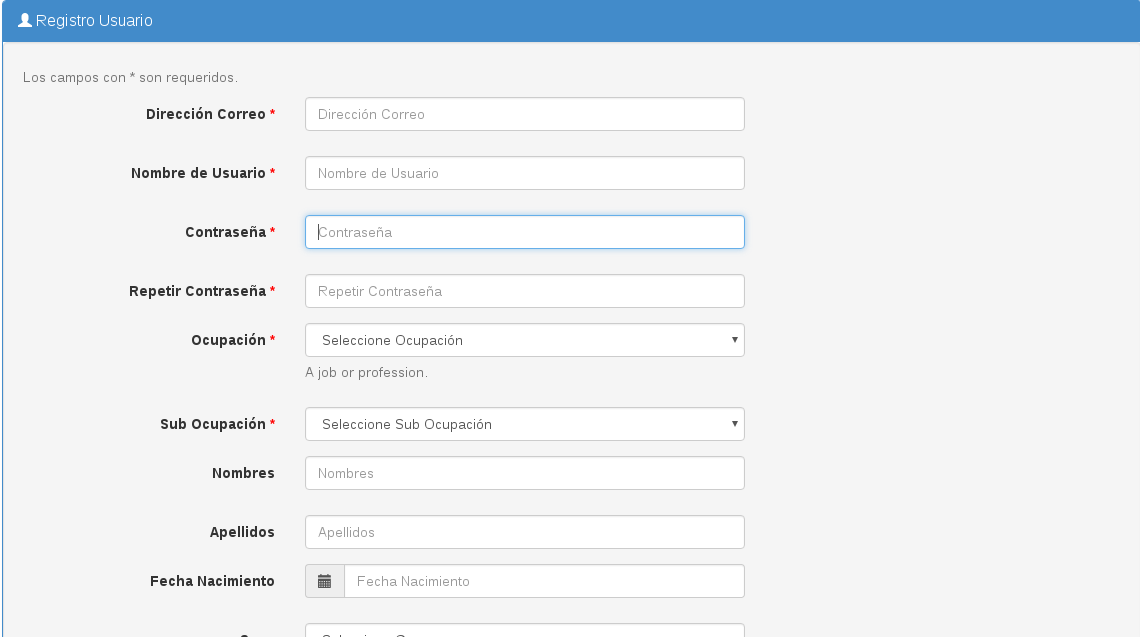
\includegraphics[scale=0.5]{userRegister}
	}	\caption{Formulario de registro de usuario de forma manual}
\end{figure}

De manera que, el sistema realiza un envió de mensaje respecto a la dirección
de correo descrita anteriormente; el mismo que implica realizar una revisión
en la bandeja de entrada o correo no deseado.

\begin{figure}[!ht]
\centering
	\fbox{
		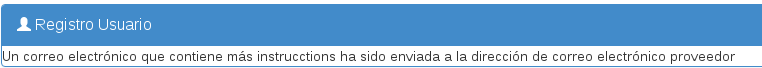
\includegraphics[scale=0.7]{successRegister}
	}	\caption{}
\end{figure}

\section{Inicio sesión de usuario} \label{sec:login}

Abra un navegador web con la siguiente dirección URL plataforma \footnote{plataforma: http://plataformaeducativalael.hum.umss.edu.bo}, pinche en el enlace \textquotedouble{Inicio Sesión},
ubicado en la parte superior derecha.

\begin{figure}[!ht]
\centering
	\fbox{
		
\includegraphics[scale=0.5]{linkLogin}
	}	\caption{Enlace de inicio sesión de usuario de forma manual}
\end{figure}

\section{Modificar datos personales}

Realizar lo siguiente definido en el sección \ref{sec:login}, a continuación, se tiene
que ingresar los datos correspondientes en los campos de Nombre Usuario:
websolutions2011, Contraseña: websolutions2011 y presionar sobre el botón
\textquotedouble{Iniciar Sesión}.

\begin{figure}[H]
\centering
	\fbox{
		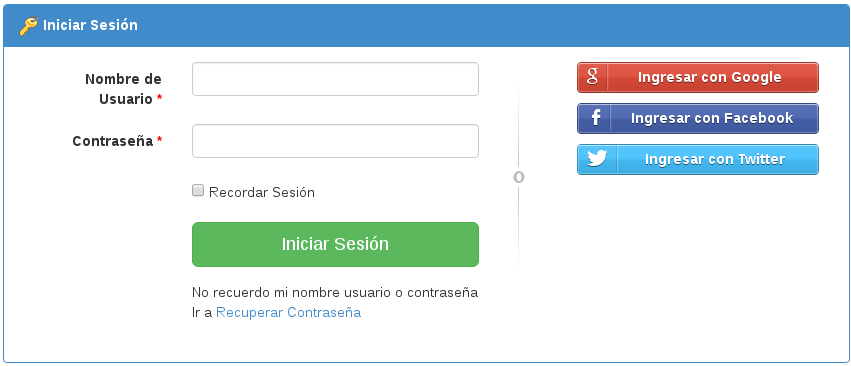
\includegraphics[scale=0.5]{formLogin}
	}	\caption{Formulario de inicio de sesión}
\end{figure}

Como se afirmo arriba, pinchar sobre la opción Perfil ubicado en la parte
superior derecha del área de trabajo.

\begin{figure}[!ht]
\centering
	\fbox{
		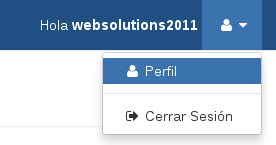
\includegraphics[scale=0.5]{linkProfile}
	}	\caption{Enlace para visualización de datos personales}
\end{figure}

Ahora veamos, la visualización de datos personales como ser de Ocupación,
Dirección de correo, Nombre de usuario y otros datos que se ingreso al momento
de su registro. 

\begin{figure}[H]
\centering
	\fbox{
		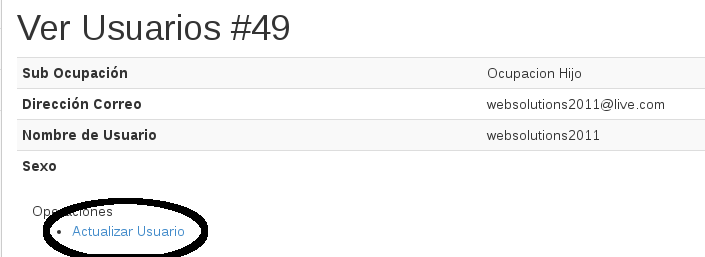
\includegraphics[scale=0.5]{viewProfile}
	}	\caption{Vista de datos personales}
\end{figure}

Así que, tiene la opción de agregar/cambiar algunos los valores del formulario
que se muestra a continuación; considerar que si cambia la dirección de correo,
tiene que realizar el procedimiento de verificación descrito en el punto 
\ref{sec:createManualUser}

\begin{figure}[H]
\centering
	\fbox{
		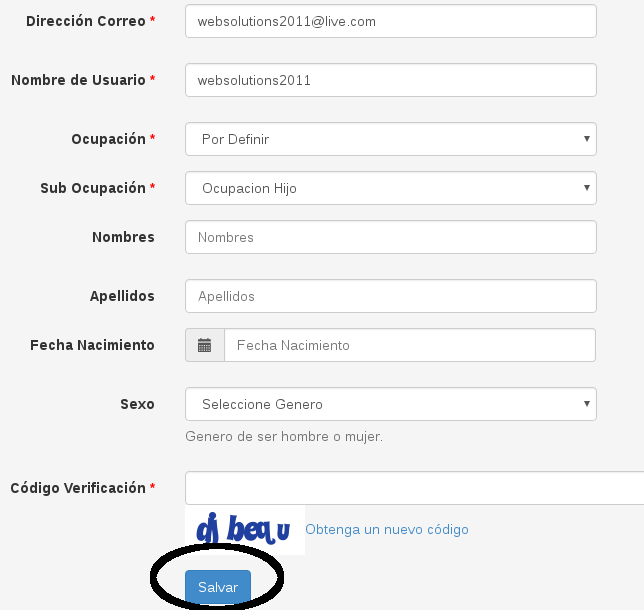
\includegraphics[scale=0.5]{formUpdateUser}
	}	\caption{Formulario de edición de datos personales de usuario}
\end{figure}

\section{Reiniciar contraseña de usuario.}

Realizar lo siguiente definido en el sección \ref{sec:login}, a continuación,
se muestra la figura de cambio de contraseña de usuario; para el mismo pinchar
sobre el enlace \textquotedouble{Recuperar Contraseña}.
  
\begin{figure}[!ht]
\centering
	\fbox{
		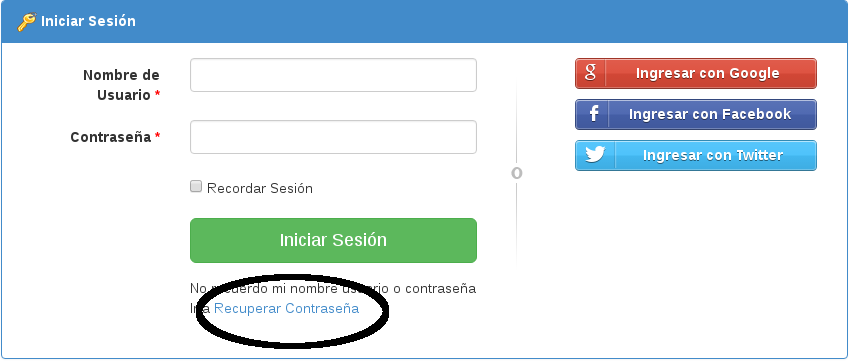
\includegraphics[scale=0.5]{linkRecoveryPassword}
	}	\caption{Enlace de recuperar contraseña de usuario}
\end{figure}

Además, llenar el siguiente formulario de solicitud de cambio de contraseña y
presionar el botón \textquotedouble{Enviar}.

\begin{figure}[H]
\centering
	\fbox{
		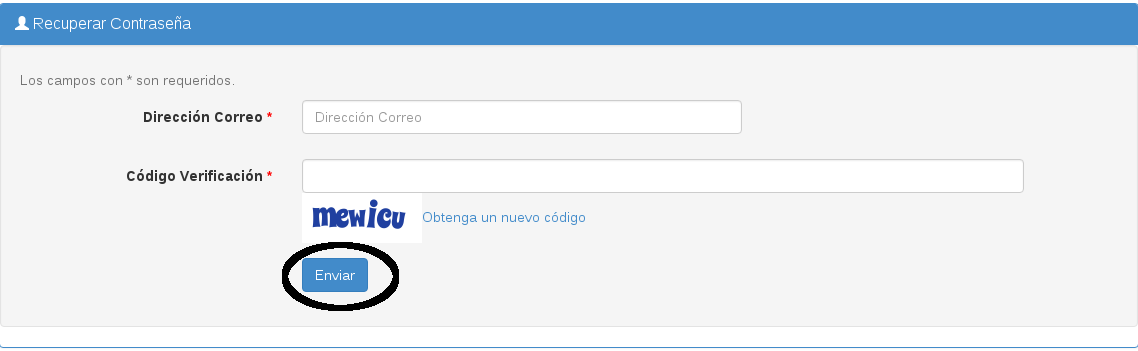
\includegraphics[scale=0.5]{formRecoveryPassword}
	}	\caption{Formulario de cambio de contraseña de usuario habilitado}
\end{figure}

Ahora veamos, de las acciones anteriores, se puede apreciar a continuación
mensaje de confirmación de envió de mensaje a bandeja de entrada.

\begin{figure}[!ht]
\centering
	\fbox{
		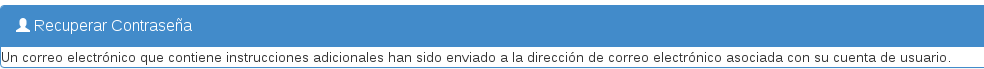
\includegraphics[scale=0.5]{successSentRecoveryPassword}
	}	\caption{Mensaje de confirmación para bandeja de entrada del usuario}
\end{figure}

Como resultado, de ingresar al cuerpo del mensaje enviado a su cuenta de correo.
Se debe pinchar sobre un enlace para proseguir con el proceso, por lo cual se
tendrá que llenar el cambio de contraseña nueva y de tal motivo finalizar.

\begin{figure}[H]
\centering
	\fbox{
		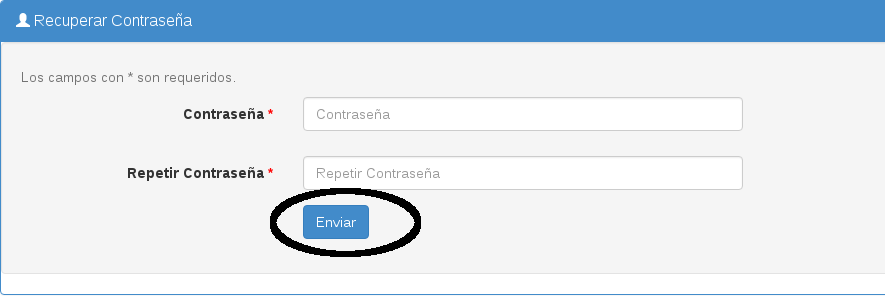
\includegraphics[scale=0.5]{formChangePassword}
	}	\caption{Formulario de cambio de contraseña}
\end{figure}


\section{Administrar Usuarios} \label{sec:manageUser}

Se considera la acción de crear a un usuario de rol autorregulado definido en
la en la sección \ref{sec:createManualUser}, para luego, realizar el uso
de inicio sesión descrito en la sección \ref{sec:login}. De manera que utilizar
las credenciales de Nombre de Usuario: administrador, Contraseña: administrador,
para luego pinchar sobre la opción \textquotedouble{Administrar Usuarios}.

\begin{figure}[!ht]
\centering
	\fbox{
		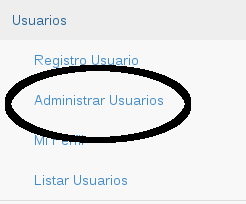
\includegraphics[scale=0.5]{linkManageUser}
	}	\caption{Enlace de administración para usuarios de sistema}
\end{figure}

\subsection{Búsqueda de usuario} \label{ssec:searchUser}

Se realiza las acciones de la sección \ref{sec:manageUser}, para luego, se
tiene que buscar al usuario con Nombre de Usuario: websolutions2011, pinchar
sobre la opción de \textquotedouble{Actualizar}. 
 
\begin{figure}[!ht]
\centering
	\fbox{
		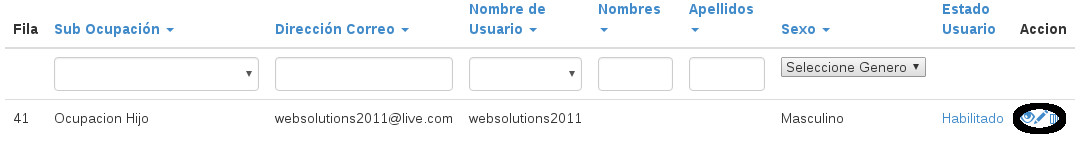
\includegraphics[scale=0.5]{linkUpdateProfileSelf}
	}	\caption{Enlace para editar perfil de usuario}
\end{figure}

\section{Gestión de rol usuario coordinador} \label{sec:manageCoordinator}


\subsection{Agregar rol coordinador}

Considerando las acciones de la sección \ref{ssec:searchUser}, veamos, que se
tenga agregar el rol de coordinador, con la adición de privilegios para poder
gestionar categorías.

\begin{figure}[!ht]
\centering
	\fbox{
		
\includegraphics[scale=0.5]{addRolCoordinator}
	}	\caption{Agregar rol coordinador a usuario}
\end{figure}

\subsection{Quitar rol coordinador}

Considerando las acciones de la sección \ref{ssec:searchUser}, a continuación,
se procede a quitar el rol de coordinador, pinchando sobre la opción 
\textquotedouble{Coordinador}.

\begin{figure}[!ht]
\centering
	\fbox{
		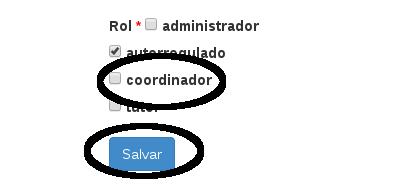
\includegraphics[scale=0.5]{removeRolCoordinator}
	}	\caption{Quitar rol coordinador a usuario}
\end{figure}


\section{Gestionar categoría}

Acerca de, la gestión de categoría se realiza el uso de las acciones descrito
en la sección \ref{sec:manageCoordinator}. Ahora se ve el inicio de sesión
descrito en la sección \ref{sec:login} utilizar las credenciales de Nombre de
Usuario: websolutions2011, Contraseña: websolutions2011.

\subsection{Registrar categoría}

A continuación pinchar sobre la opción \textquotedouble{Registrar Categoría}.

\begin{figure}[!ht]
\centering
	\fbox{
		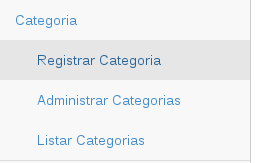
\includegraphics[scale=0.5]{linkCreateCategory}
	}	\caption{Enlace para crear una categoría nueva}
\end{figure}

\begin{itemize}

\item \textbf{Categoría padre}

A continuación, se tiene que realizar la creación de una categoría denominada
como \textquotedouble{padre}; seleccionar la opción mencionada, el cual puede
contener categorías hijas; se puede apreciar el llenado de campos en la
siguiente figura.

\begin{figure}[!ht]
\centering
	\fbox{
		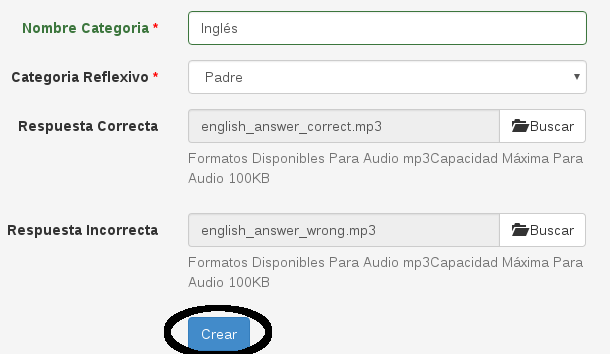
\includegraphics[scale=0.5]{formCategoryFather}
	}	\caption{Formulario de llenado para categoría padre}
\end{figure}

\item \textbf{Categoría hija}

Dicho lo anterior, se debe crear una categoría denominada de igual manera como
\textquotedouble{hija}; seleccionar la opción mencionada, el mismo que se
refiere concreta mente al programa de aprendizaje que contiene a los podcasts.

\begin{figure}[!ht]
\centering
	\fbox{
		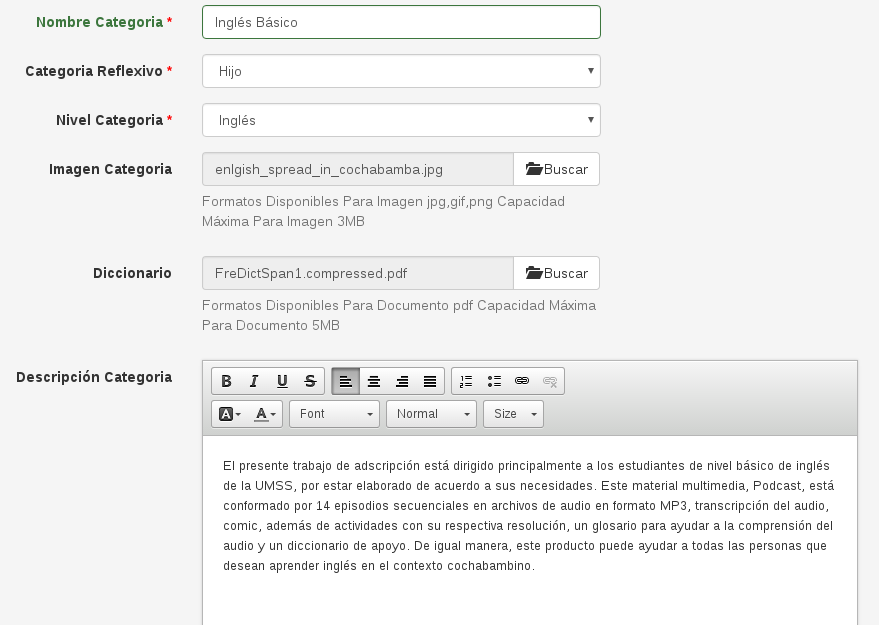
\includegraphics[scale=0.5]{formCategoryChild}
	}	\caption{Formulario de llenado para categoría hija}
\end{figure}
\end{itemize}


 \subsection{Actualizar categoría}

A continuación pinchar sobre la opción \textquotedouble{Administrar Categorías}.

\begin{figure}[!ht]
\centering
	\fbox{
		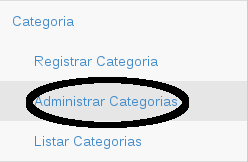
\includegraphics[scale=0.5]{linkUpdateCategory}
	}	\caption{Enlace para editar una categoría registrada}
\end{figure}

\begin{itemize}

\item \textbf{Categoría padre}

Hecha esta salvedad, se tiene que seleccionar la categoría padre,
\textquotedouble{Inglés Básico}, pinchar sobre la opción actualizar.

\begin{figure}[!ht]
\centering
	\fbox{
		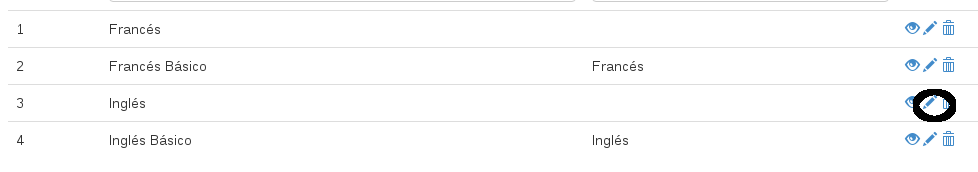
\includegraphics[scale=0.5]{linkUpdateCategoryFather}
	}	\caption{Enlace para editar una categoría padre}
\end{figure}

A continuación, se presenta el formulario de actualización de los campos
que pueden ser sujetos a cambio: Nombre Categoría o Respuesta Correcta o
Respuesta Incorrecta.

\begin{figure}[!ht]
\centering
	\fbox{
		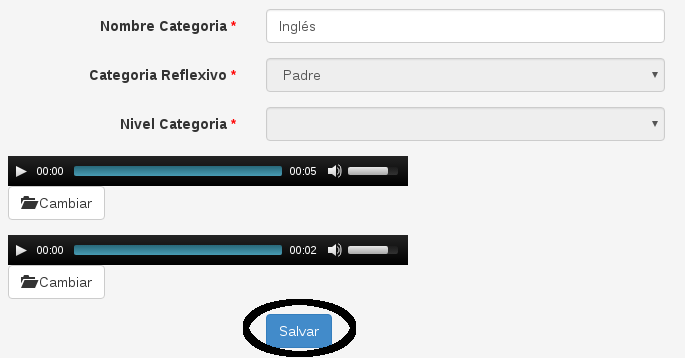
\includegraphics[scale=0.5]{formUpdateCategoryFather}
	}	\caption{Formulario de edición para categoría padre}
\end{figure}

\item \textbf{Categoría hija}

Consideremos ahora, una categoría hija por la característica en la columna
de \textquotedouble{Nivel Categoría}, la misma referencia a un nombre de
categoría; a continuación pinchar sobre la opción \textquotedouble{Actualizar}.

\begin{figure}[!ht]
\centering
	\fbox{
		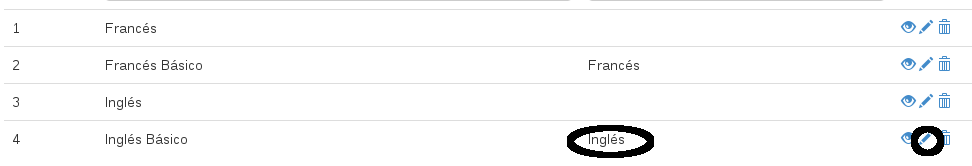
\includegraphics[scale=0.5]{linkUpdateCategoryChild}
	}	\caption{Enlace para editar una categoría hija}
\end{figure}

\end{itemize}

Luego, se puede realizar el cambio de alguno de los campos como ser: Nombre
Categoría o Nivel Categoría o Imagen Actual o Diccionario o Descripción o
Créditos u Objetivos. 

\begin{figure}[!ht]
\centering
	\fbox{
		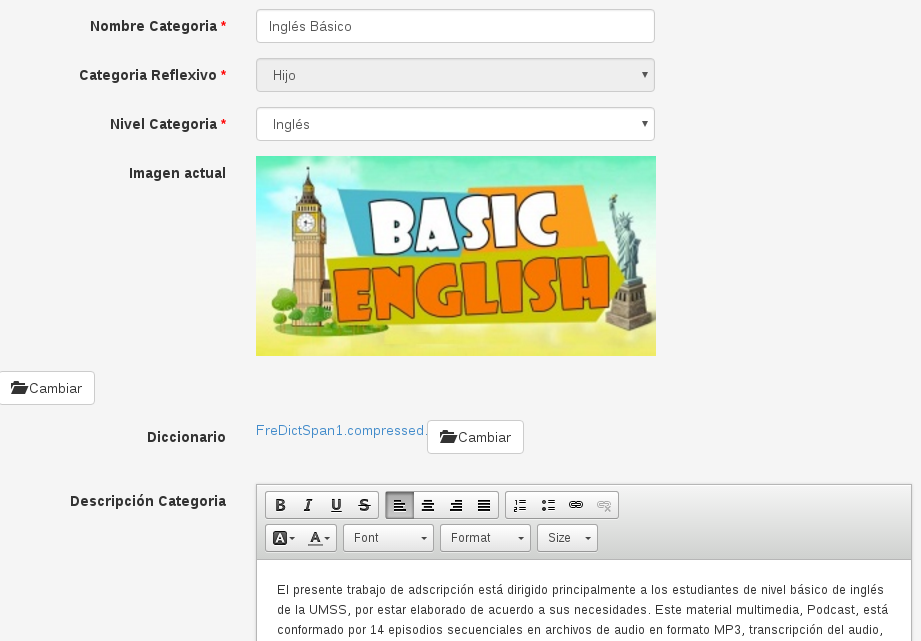
\includegraphics[scale=0.5]{formUpdateCategoryChild}
	}	\caption{Formulario de edición para categoría hija}
\end{figure}

\subsection{Quitar categoría}

Considerar la dependencia existente entre una categoría padre y categoría hija;
quiere decir, si desea eliminar una categoría padre, previamente tiene que
eliminar una categoría hija.

\begin{itemize}

\item \textbf{Categoría hija}

A menos que, categoría hija no tenga asignado uno o más podcast, se puede
continuar con la eliminación.

\begin{figure}[!ht]
\centering
	\fbox{
		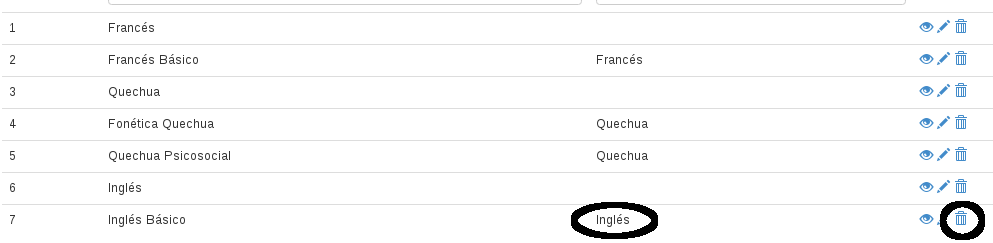
\includegraphics[scale=0.5]{linkDeleteCategoryChild}
	}	\caption{Enlace eliminar para categoría hija}
\end{figure}

\item \textbf{Categoría padre}

A no ser que, categoría padre no tenga asignado una o más categorías, el sistema
permite la eliminación de la misma.

\begin{figure}[!ht]
\centering
	\fbox{
		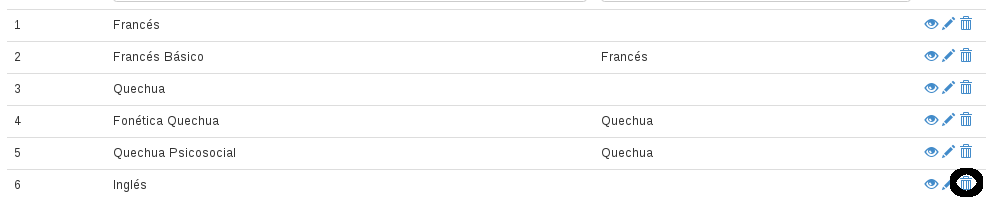
\includegraphics[scale=0.5]{linkDeleteCategoryFather}
	}	\caption{Enlace eliminar para categoría padre}
\end{figure}

\end{itemize}

\section{Gestión rol usuario tutor}

\subsection{Agregar rol tutor}

Se realiza las acciones de la sección \ref{sec:manageUser}, para luego, se
tenga agregar el rol de coordinador, con la adición de privilegios para poder
gestionar contenido.

\begin{figure}[!ht]
\centering
	\fbox{
		
\includegraphics[scale=0.5]{addRolTutor}
	}	\caption{Agregar rol tutor a usuario}
\end{figure}

\subsection{Quitar rol tutor}

Considerando las acciones de la sección \ref{ssec:searchUser}, a continuación,
se realiza pinchar sobre el rol \textquotedouble{Tutor} y pinchar sobre el botón
salvar.

\begin{figure}[!ht]
\centering
	\fbox{
		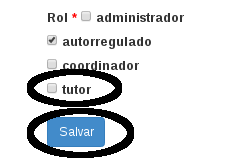
\includegraphics[scale=0.6]{removeRolTutor}
	}	\caption{Quitar rol coordinador a usuario}
\end{figure}

\section{Gestionar contenido}

Acerca de, el inicio de sesión descrito en la sección \ref{sec:login}, utilizar
las credenciales de Nombre de Usuario: websolutions2011, Contraseña: websolutions2011.

\subsection{Registrar contenido}

\begin{figure}[!ht]
\centering
	\fbox{
		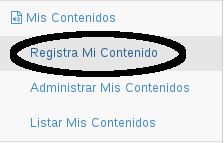
\includegraphics[scale=0.5]{linkCreateContent}
	}	\caption{Enlace para crear un podcast nuevo}
\end{figure}

Dicho lo anterior, llenar los siguientes campos de Título, Imagen, Reproductor,
Fecha de liberación, Resumen, Resolución, Glosario, Créditos y presionar sobre
el botón \textquotedouble{Crear}.

\begin{figure}[!ht]
\centering
	\fbox{
		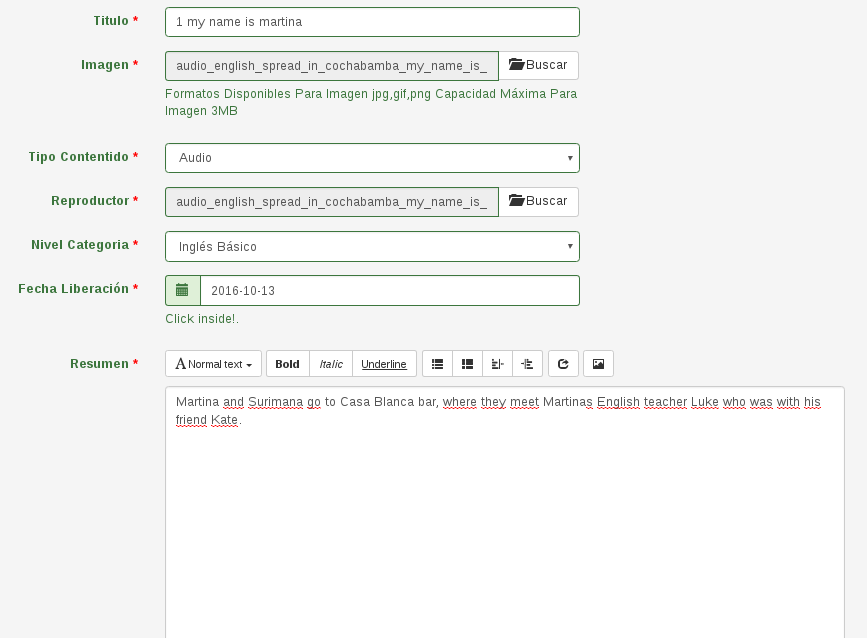
\includegraphics[scale=0.5]{formCreateContent}
	}	\caption{Formulario de registro de podcast}
\end{figure}

\subsection{Habilitar contenido de forma manual} \label{ssec:availableContent}

Ahora veamos, se realiza la continuación la manera de dar de alta a un contenido;
de manera que pueda estar disponible en la parte pública del sistema.

\begin{figure}[H]
\centering
	\fbox{
		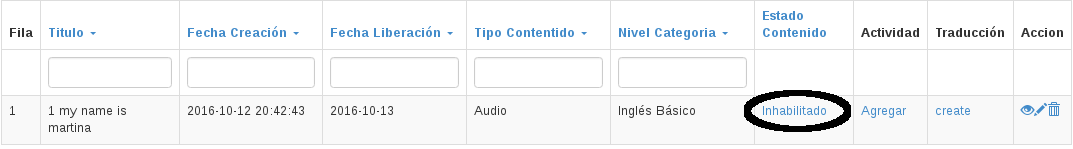
\includegraphics[scale=0.5]{linkAvailableContent}
	}	\caption{Enlace para habilitar contendido}
\end{figure}

\subsection{Actualizar mis contenido}

A continuación pinchar sobre la opción \textquotedouble{Administrar Mis Contenidos}.

\begin{figure}[!ht]
\centering
	\fbox{
		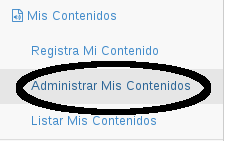
\includegraphics[scale=0.5]{linkUpdateContent}
	}	\caption{Enlace para editar un podcast registrado}
\end{figure}

También, se tiene que seleccionar el podcast a editar 
\textquotedouble{1 my name is martina}, pinchar sobre la opción actualizar.
 
\begin{figure}[!ht]
\centering
	\fbox{
		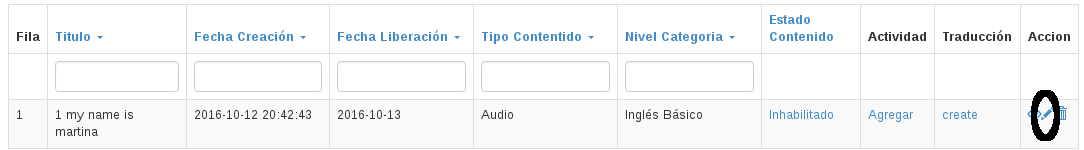
\includegraphics[scale=0.5]{linkUpdateChooseContent}
	}	\caption{Enlace para editar un podcast específico}
\end{figure}

Hay que mencionar, se puede realizar el cambio de los campos de Título o Imagen o
Reproductor o Nivel Categoría o Fecha liberación o Resumen o Resolución o Glosario
o Créditos y presionar el botón \textquotedouble{Salvar}.

\begin{figure}[H]
\centering
	\fbox{
		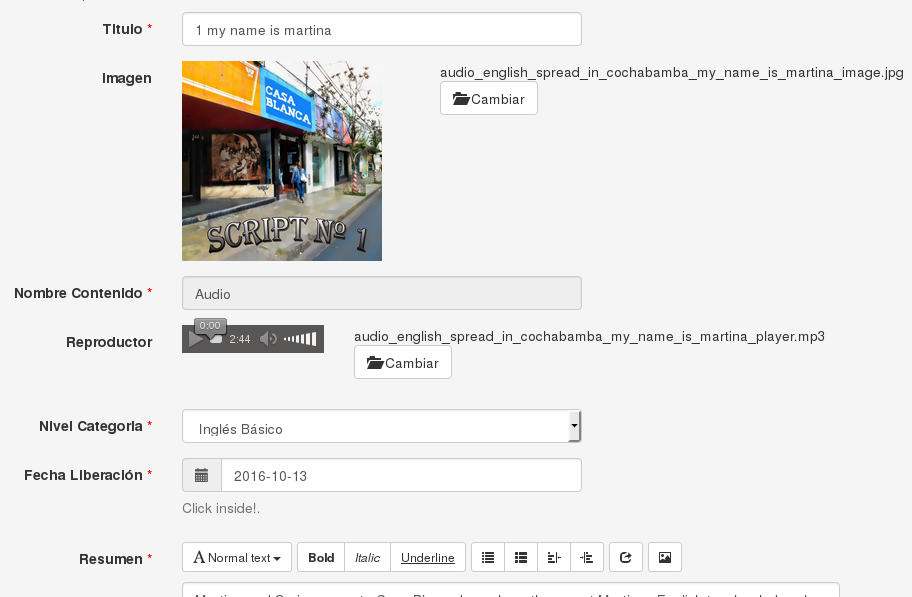
\includegraphics[scale=0.5]{formUpdateContent}
	}	\caption{Formulario de edición de contendido}
\end{figure}

\subsection{Quitar contenido}

A menos que, el contenido no tenga la dependencia de actividades de tipo 
cotejamiento, comprensión puede darse la eliminación.

\begin{figure}[!ht]
\centering
	\fbox{
		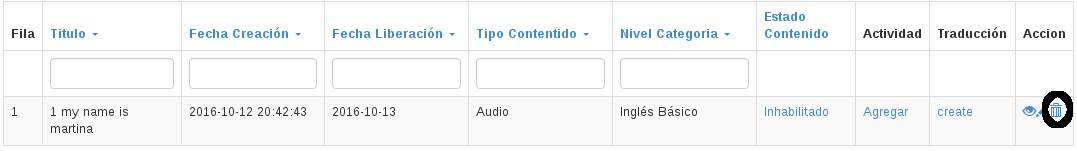
\includegraphics[scale=0.5]{linkDeleteContent}
	}	\caption{Enlace para eliminar contendido}
\end{figure}

\section{Gestionar suscripción}

Con tal que, visualizar la disposición de un podcast, se debe proseguir con
la siguiente manera, caso contrario realizar la acción definido en la sección
\ref{ssec:availableContent}.

Realizar el uso de inicio sesión descrito en la sección \ref{sec:login}, utilizar
las credenciales de Nombre de Usuario: websolutions2011, Contraseña:
websolutions2011.

\begin{figure}[!ht]
\centering
	\fbox{
		
\includegraphics[scale=0.5]{linkMainPage}
	}	\caption{Enlace para visualización para acceso a parte pública}
\end{figure}

Consideremos ahora, el ingresar para la parte pública del sistema y dar
continuidad, pinchando sobre el enlace ubicado en el menú principal de la
parte publica, realizando la elección de la categoría \textquotedouble{Inglés}.

\begin{figure}[!ht]
\centering
	\fbox{
		
\includegraphics[scale=0.5]{linkCategoryMainPage}
	}	\caption{Enlace de visualización de categoría hija}
\end{figure}

\subsection{Panel administrativo} \label{ssec:dashboard}

Consideremos ahora, la verificación del registro de la suscripción ingresando
al panel administrativo de usuario.

\begin{figure}[!ht]
\centering
	\fbox{
		
\includegraphics[scale=0.5]{linkDashboard}
	}	\caption{Enlace de acceso a panel administrativo}
\end{figure}

Llegados a este punto, presionar sobre el enlace \textquotedouble{Administrar
Mis Suscripciones}; para apreciar el registro de suscripción de una categoría.

\begin{figure}[!ht]
\centering
	\fbox{
		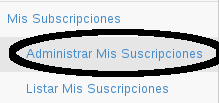
\includegraphics[scale=0.5]{linkManageSubscription}
	}	\caption{Enlace de administración mis suscripciones}
\end{figure}

\begin{itemize}

\item \textbf{Suscripción}

Dicho lo anterior, se aprecia la categoría hija, de la misma se puede pinchar sobre
el botón \textquotedouble{Suscribirse}; de esa forma en el tiempo se realizara un
envió de notificación por vía correo electrónico de la disposición de nuevo material
disponible.

\begin{figure}[!ht]
\centering
	\fbox{
		
\includegraphics[scale=0.5]{buttonAddSubscription}
	}	\caption{Botón de agregación de suscripción}
\end{figure}

Por todo esto, se realiza las observaciones descritas en la sección
\ref{ssec:dashboard}, se puede visualizar el registro.  

\begin{figure}[!ht]
\centering
	\fbox{
		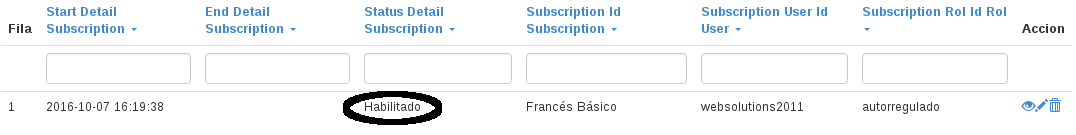
\includegraphics[scale=0.5]{viewManageAvailableSubscription}
	}	\caption{vista administrativa de suscripción de categorías}
\end{figure}

\item \textbf{Dar de baja}

Antes de examinar, se realiza la acción necesaria para dar de baja una
suscripción registrada, de forma que se debe pinchar sobre el botón 
\textquotedouble{Suscrito}.

\begin{figure}[!ht]
\centering
	\fbox{
		
\includegraphics[scale=0.5]{buttonDeleteSubscription}
	}	\caption{Botón para eliminar suscripción}
\end{figure}

Como se afirmo arriba, se realiza las observaciones descritas en la sección
\ref{ssec:dashboard}, realizar la verificación correspondiente de la acción
de baja de suscripción.  

\begin{figure}[!ht]
\centering
	\fbox{
		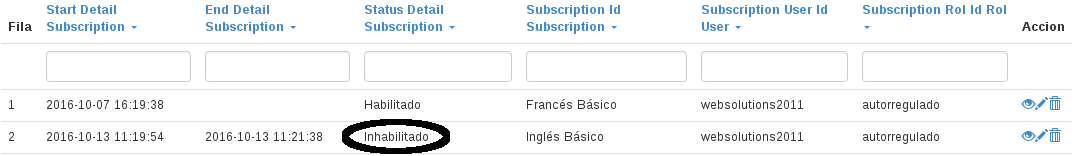
\includegraphics[scale=0.5]{viewManageUnavailableSubscription}
	}	\caption{vista administrativa de suscripción de categorías}
\end{figure}

\end{itemize}

\section{Gestionar transcripción}

A su vez, se ve el inicio de sesión descrito en la sección \ref{sec:login}, hacer
uso de las credenciales Nombre de Usuario: websolutions2011, Contraseña: 
websolutions2011,

A continuación pinchar sobre la opción \textquotedouble{Administrar Mis Contenidos}.

\begin{figure}[!ht]
\centering
	\fbox{
		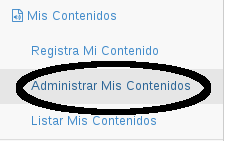
\includegraphics[scale=0.5]{linkUpdateContent}
	}	\caption{Enlace para editar un podcast registrado}
\end{figure} 

También, se tiene que seleccionar el podcast 
\textquotedouble{1 en dehors de l'immigration} para agregar un glosario,
pinchar sobre la opción \textquotedouble{create} de la columna
\textquotedouble{Traducción}.
 
\begin{figure}[!ht]
\centering
	\fbox{
		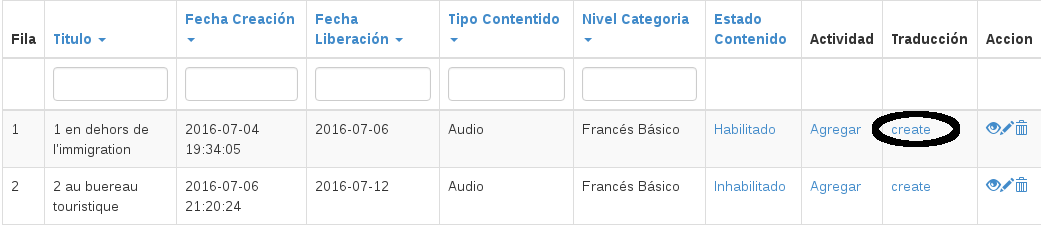
\includegraphics[scale=0.5]{linkCreateTranslation}
	}	\caption{Enlace para crear una transcripción}
\end{figure}

\begin{itemize}

\item \textbf{Glosario}

Mas aun, se debe seleccionar el Tipo de Transcripción en Glosario y a continuación
ingresar los datos para Frase, Lenguaje, Descripción y por último pinchar sobre el
botón \textquotedouble{Crear}.
 
\begin{figure}[!ht]
\centering
	\fbox{
		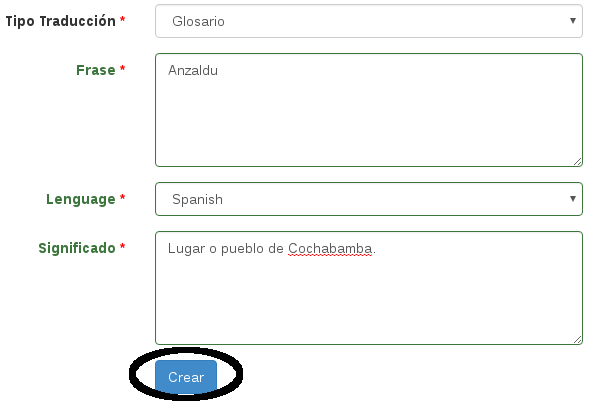
\includegraphics[scale=0.5]{formCreateGlossary}
	}	\caption{Formulario de registro de transcripción de tipo glosario}
\end{figure}

\item \textbf{Subtitulado}

Mas aun, se debe seleccionar el Tipo de Transcripción en Glosario y a continuación
ingresar los datos para Frase, Lenguaje, Descripción y por último pinchar sobre el
botón \textquotedouble{Crear}.

En otras palabras, utilizar el reproductor de audio para establecer los campos de
Tiempo Inicio y Tiempo Final, caso contrario pinchar sobre el botón 
\textquotedouble{Reajustar Reproductor}.

\begin{figure}[!ht]
\centering
	\fbox{
		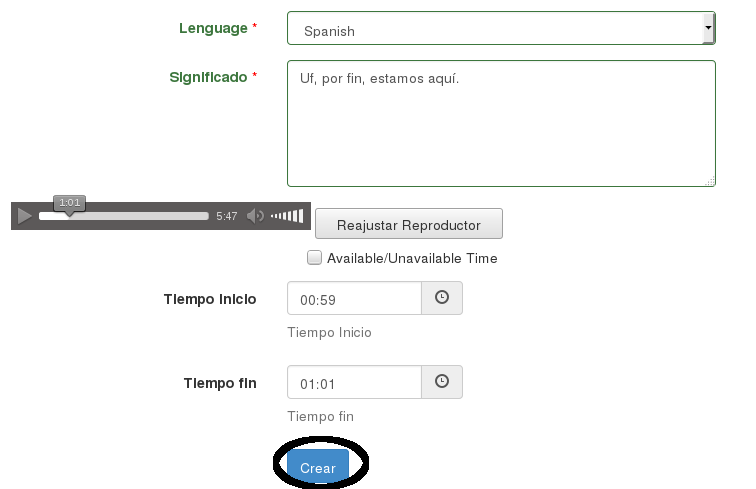
\includegraphics[scale=0.5]{formCreateLyric}
	}	\caption{Formulario de registro de transcripción de tipo subtitulado}
\end{figure}

\end{itemize}



\end{document}